\documentclass[11pt]{article}
\usepackage{graphicx}

\usepackage{hyperref}

\graphicspath{{figs/}, {doc/}}
\newcommand{\tempS}[1]{#1}
\newcommand{\twowidth}{6in}


\usepackage[plain]{fancyref}

\title{Plots for \texttt{dfo-bb046-20200717}}
\author{Jody M.\ Klymak}

\begin{document}

\maketitle 

\section{Location and timing}

Seaglider \texttt{dfo-bb046} was launched from QCS02 on 17 July, 2020 by Chris O'Sullivan and co-workers at Hakai.  The glider transited southwest along the line in \fref{fig:MissionMap}.  There is a Marine Protected Area between stations marked MPA1 and MPA2, and during the first line, the glider was held to going no deeper than 140 m.  The first line was continued offshore, before turning for the second Line.  This line skirted the north side of the MPA (as did the next two), allowing us to go to the bottom.  The glider was turned just before the station SS5, and did another line to the station marked "Shelf", and then the glider returned to almost QCS02.  It was recovered by Chris O'Sullivan and Jody Klymak, with Nick driving the boat from the Good Hope VI on Aug 6, 2020.  

\begin{figure*}[htbp]
  \begin{center}
    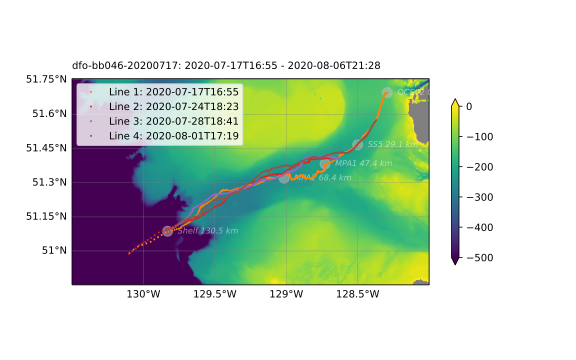
\includegraphics[width=\twowidth]{MissionMap}
    \caption{      
      \label{fig:MissionMap} }
  \end{center}
\end{figure*}

Piloting was generally quite good.  We used the new waypoint planning software from Alseamar on Glimpse, and that seemed to work well. The glider doesn't turn underwater, so that is a drawback.  We also tried, but eventually turned off, their heading correction.  This correction was just by heading mismatch, and that was deemed untenable for tidal currents. 

\section{Property plots}

We do a crude de-tiding procedure here to remove the isopycnal heave due to the tide, but still retain the large-scale isopycnal tilts.  For each cast, we over-interpolate the scalars onto an isopycnal grid, and we also determine the depth of each isopycnal in the grid.  The depths of those isopycnals are then each smoothed in time; right now its a 30-point boxcar convolution.  Should probably be redone properly in the time domain, but this is really just qualitative.  A depth-time map is then easy to make by interpolating each cast back in space from these smoothed isopycnal depths.  An example is shown in \fref{fig:TempAnom}.  

There are a few things worth noting. First, the canyon is significantly less stratified than the water above.  This stratification difference persists offshore, but speaks to the difference between the upper ocean water and deeper.  

Isopycnal tilts are interesting.  The $\sigma_{\theta}=26\ \mathrm{kg\,m^{-3}}$ isopycnal bws up a bit from the ocean, and then drops towards the head of the canyon.  There is a further uplift towards QCS02, but we shuld be careful to note this is to the north.  Conversely, the $\sigma_{\theta}=26\ \mathrm{kg\,m^{-3}}$ tilts upwards towards the head.  

 

\begin{figure*}[htbp]
  \begin{center}
    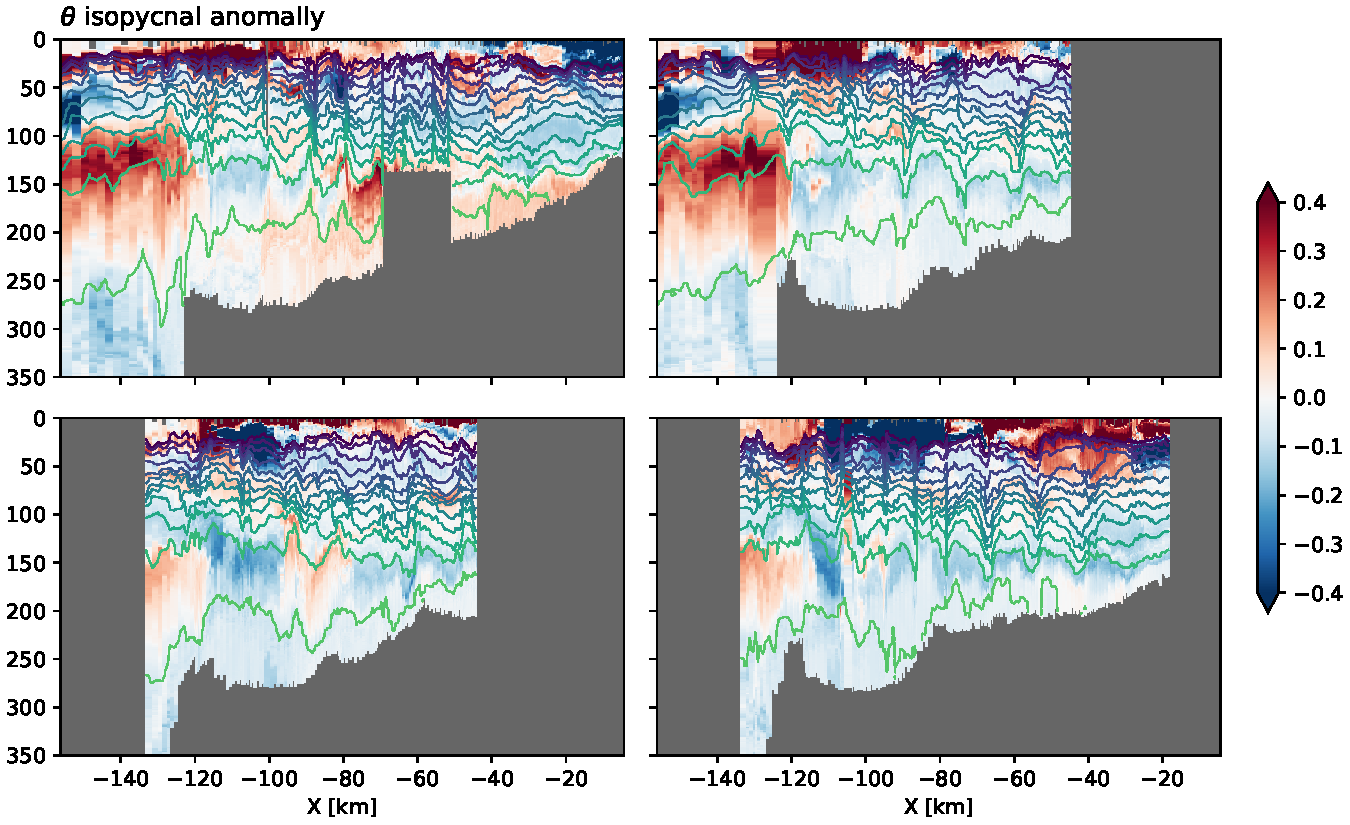
\includegraphics[width=\textwidth]{TempAnom.pdf}
        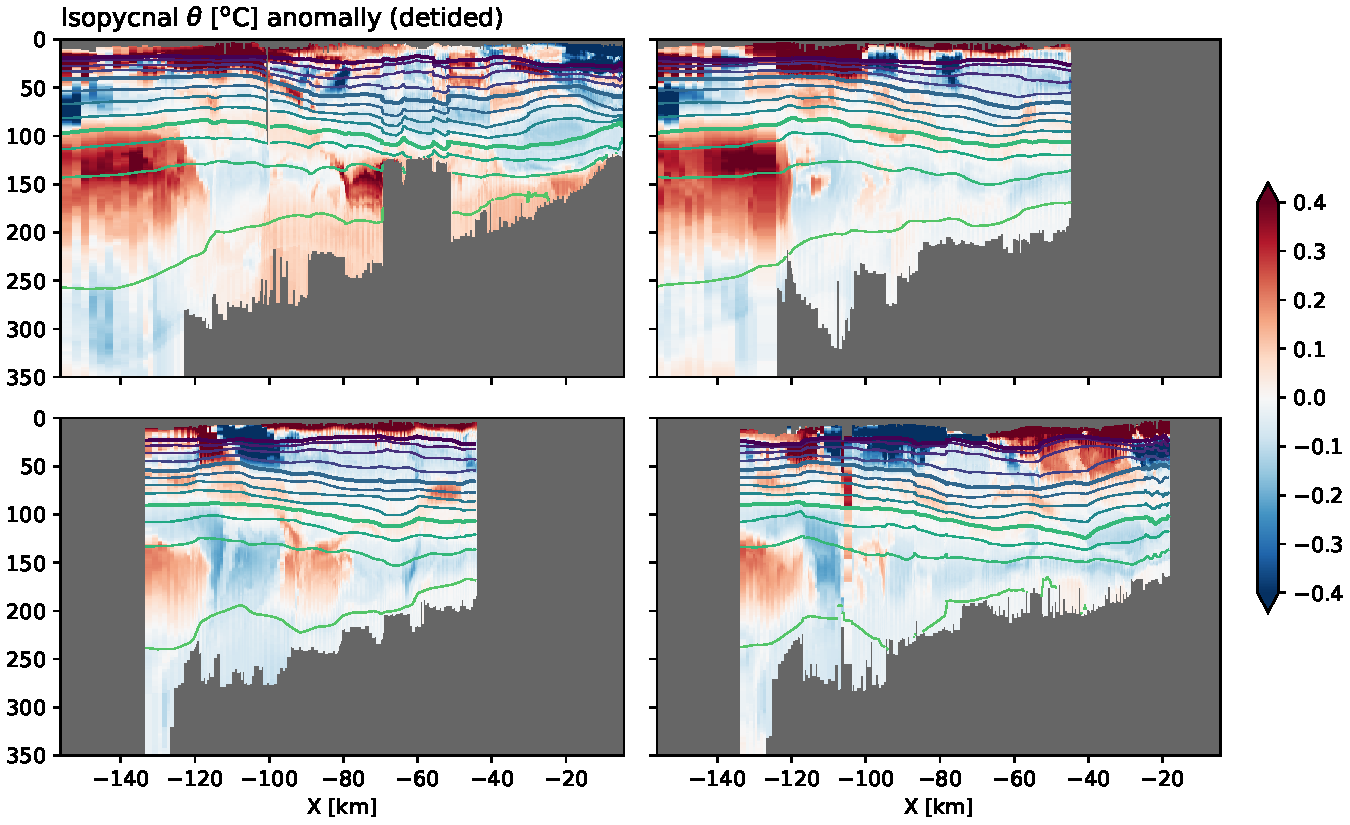
\includegraphics[width=\textwidth]{TempAnomDetide}
    \caption{Isopycnal temperature anomaly (relative to deployment mean).  Contours are constant density, with the thick contours $\sigma_{\theta} = 24, 25, 26\ \mathrm{kg\,m^{-3}}$. The bottom sets of plots have  
      \label{fig:TempAnom} }
  \end{center}
\end{figure*}

In terms of water properties, there is a mass of warm water between 26 and 26.75 in the open ocean (\fref{fig:TempAnom}).  There are signs of very similar water in the first occupation, and an attenuated version the third pass.  The warm water carries  also high-O2 water with it (\fref{fig:O2Detide}).  

Overall, it appears there is substantial mixing in the canyon. It mixes the the temperature anomalies away on the scale of less than a week, and it mixes low-oxygen water up in the water column. There is also evidence that the amount of water denser than 26.75 decreases during the mission.  

The picture from T-S plots is consistent with mixing.  The ocean water appears as a knee in the T-S plot (\fref{fig:TSCanyon}).  We see on the second pass that the knee is almost completely absent in the canyon, but on the third pass it has returned for some locations.  For the last pass the T-S curve tightens even further. 

There are also interesting interleaving features in the upper water column, with slanted temperature anomallies in the upper 100 km indicative of stirring (\fref{fig:TempAnom}).   

\begin{figure*}[htbp]
  \begin{center}
    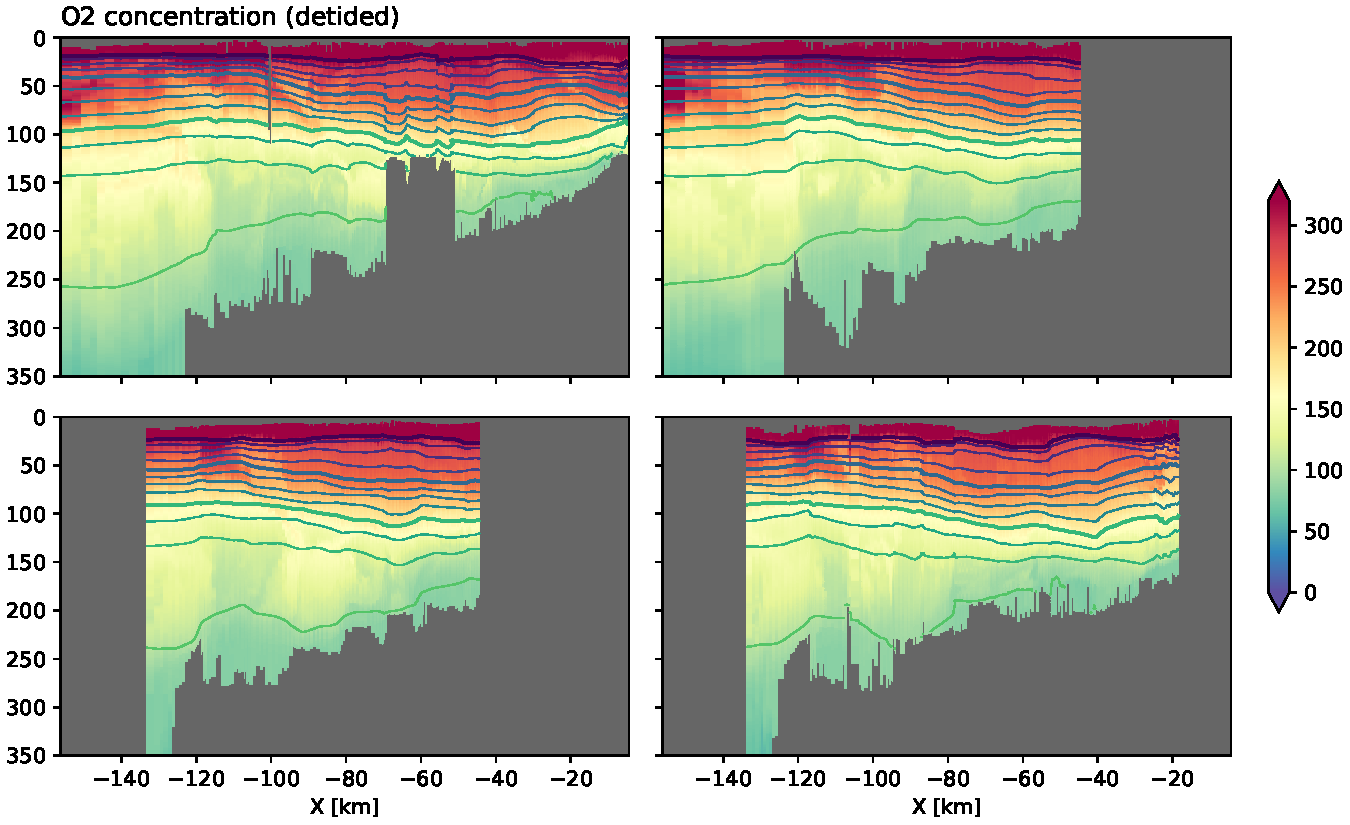
\includegraphics[width=\textwidth]{O2Detide}
    \caption{
      \label{fig:O2Detide} }
  \end{center}
\end{figure*}

\begin{figure*}[htbp]
  \begin{center}
    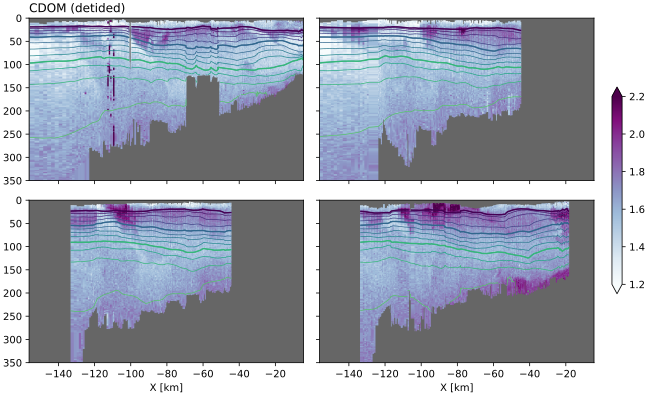
\includegraphics[width=\textwidth]{CDOMDetide}
    \caption{
      \label{fig:CDOMDetide} }
  \end{center}
\end{figure*}

\begin{figure*}[htbp]
  \begin{center}
    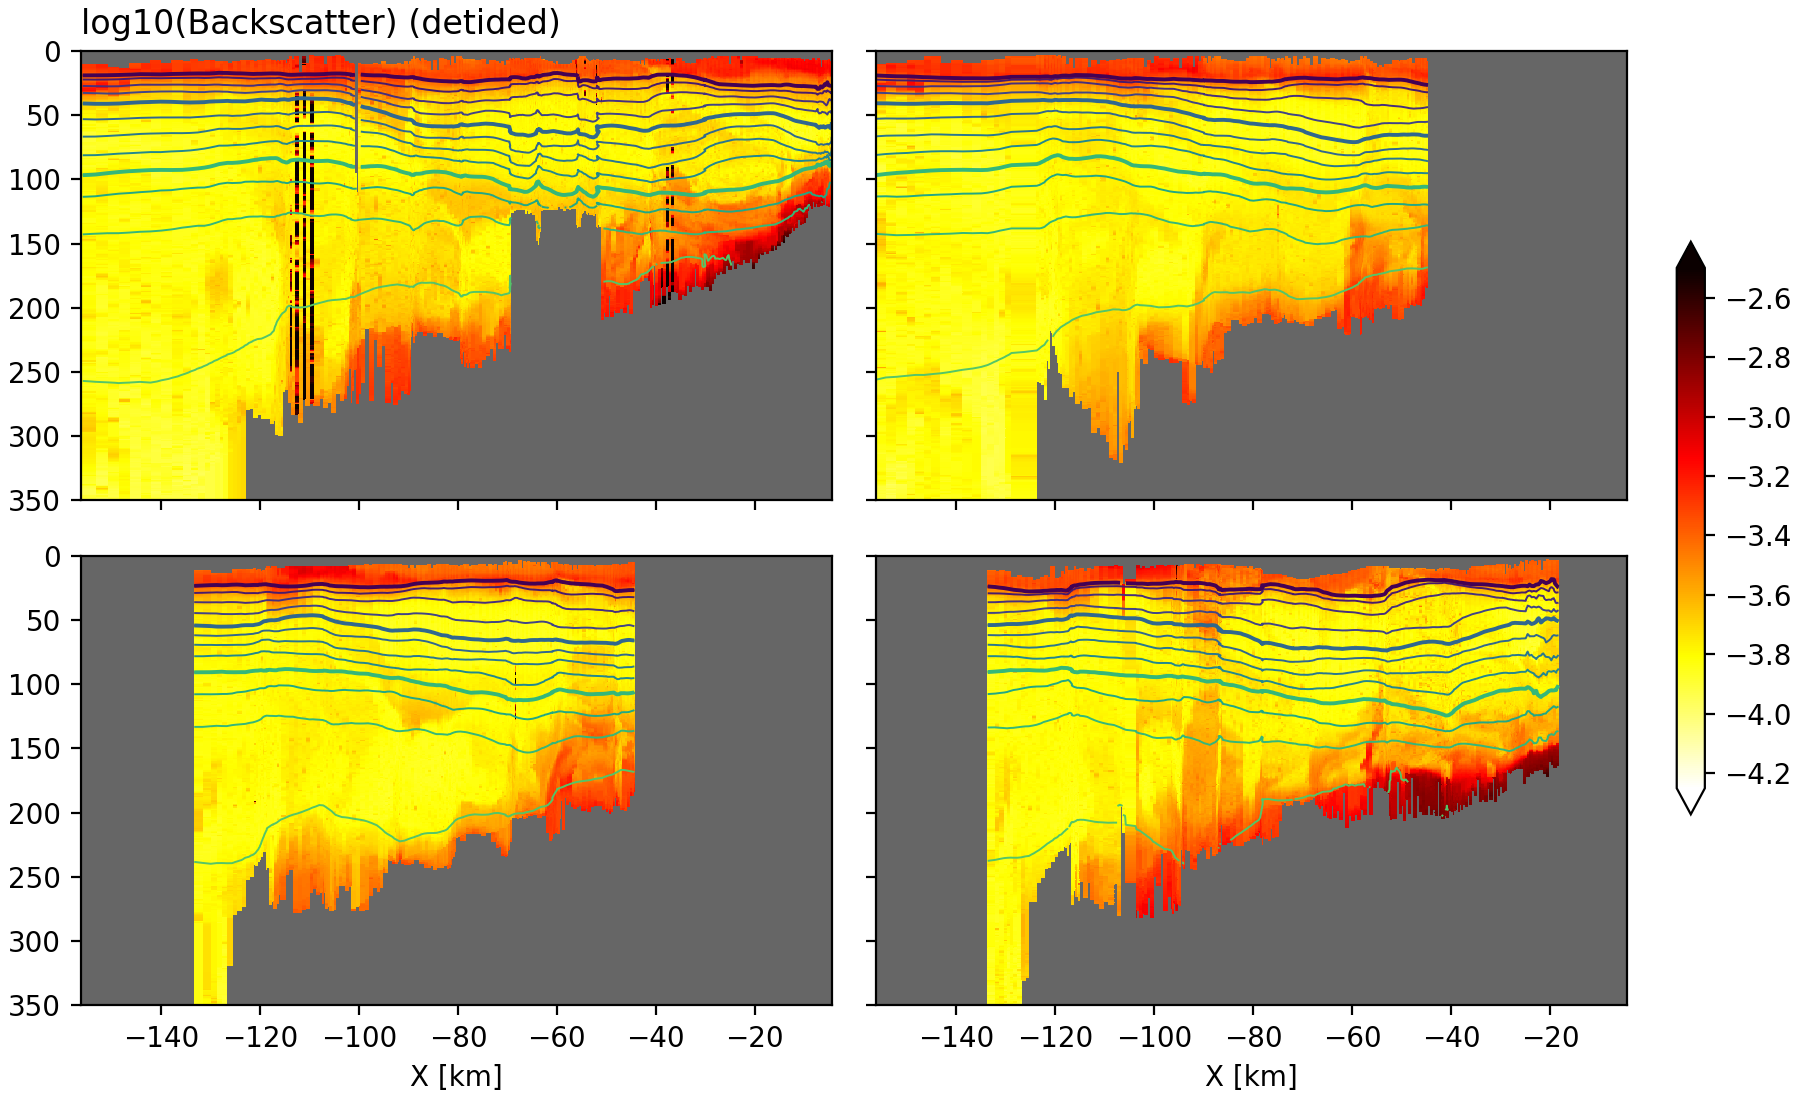
\includegraphics[width=\textwidth]{BackscatterDetide}
    \caption{
      \label{fig:BackscatterDetide} }
  \end{center}
\end{figure*}

\begin{figure*}[htbp]
  \begin{center}
    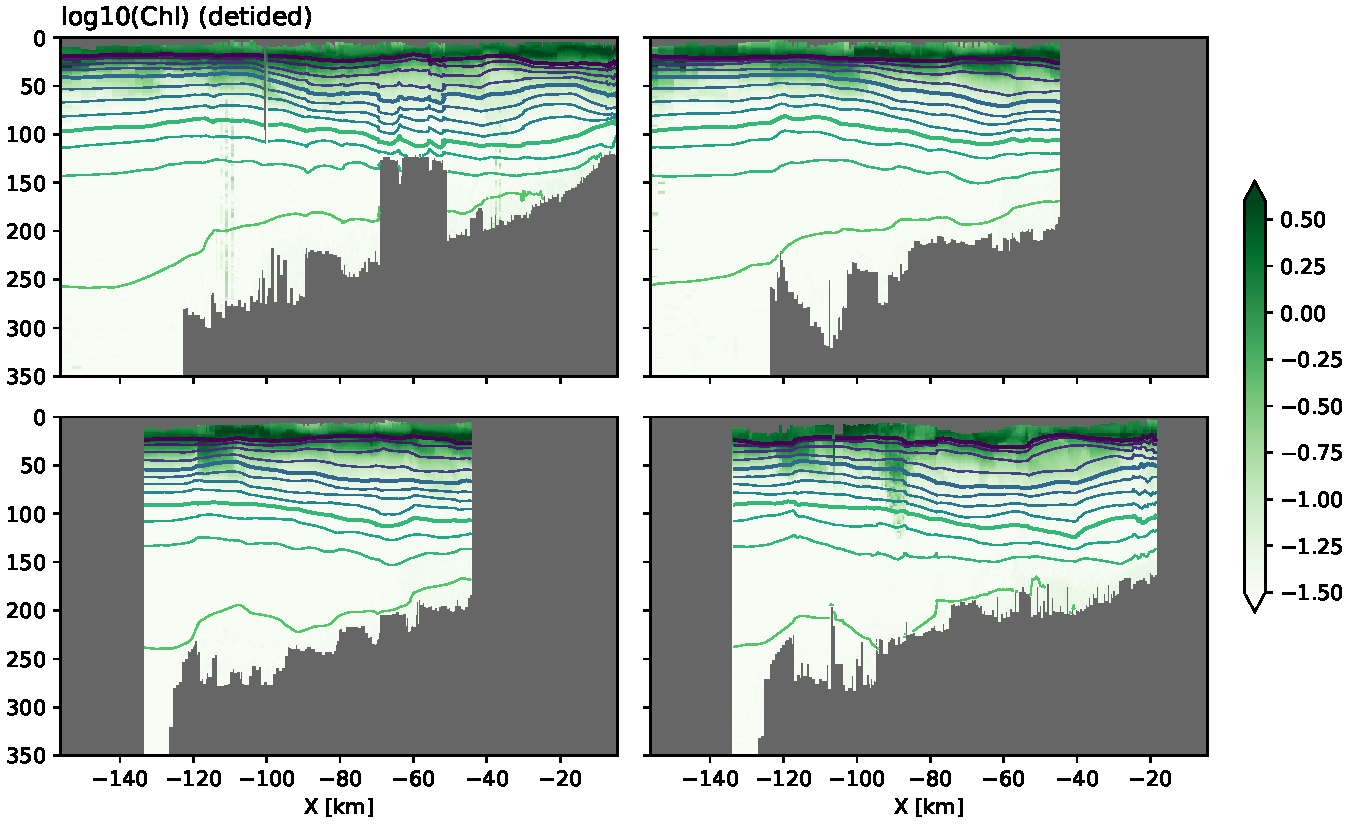
\includegraphics[width=\textwidth]{ChlDetide}
    \caption{
            \label{fig:ChlDetide} }
  \end{center}
\end{figure*}

\begin{figure*}[htbp]
  \begin{center}
    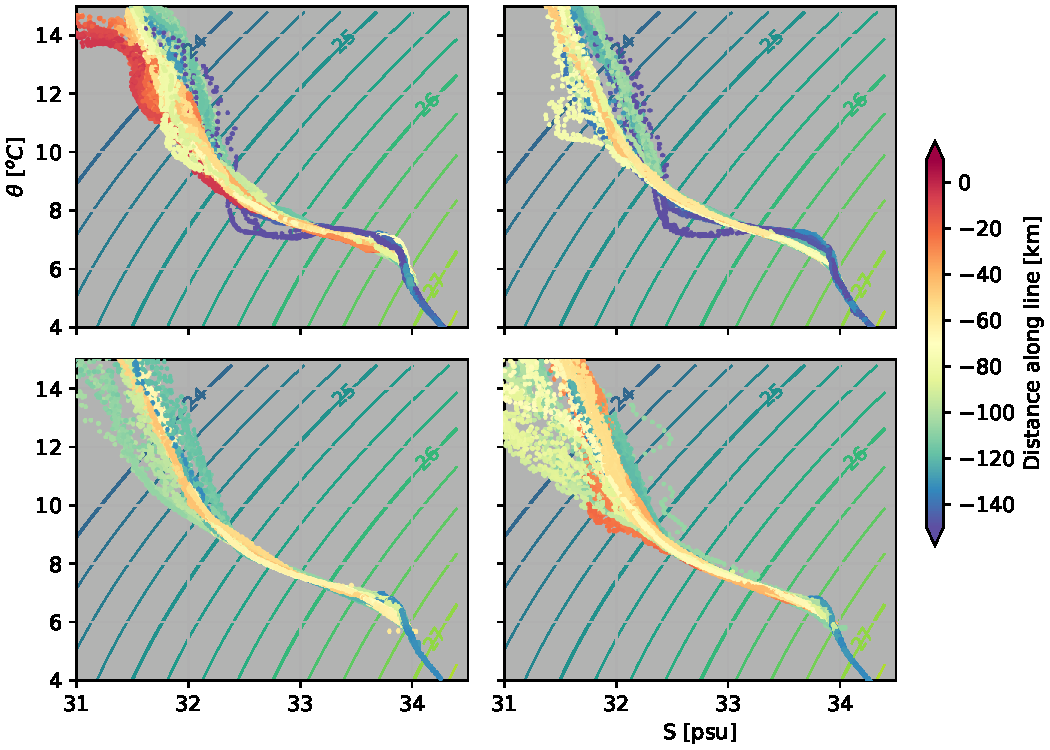
\includegraphics[width=\twowidth]{TSAll}
    \caption{
      \label{fig:TSAll} }
  \end{center}
\end{figure*}

\begin{figure*}[htbp]
  \begin{center}
    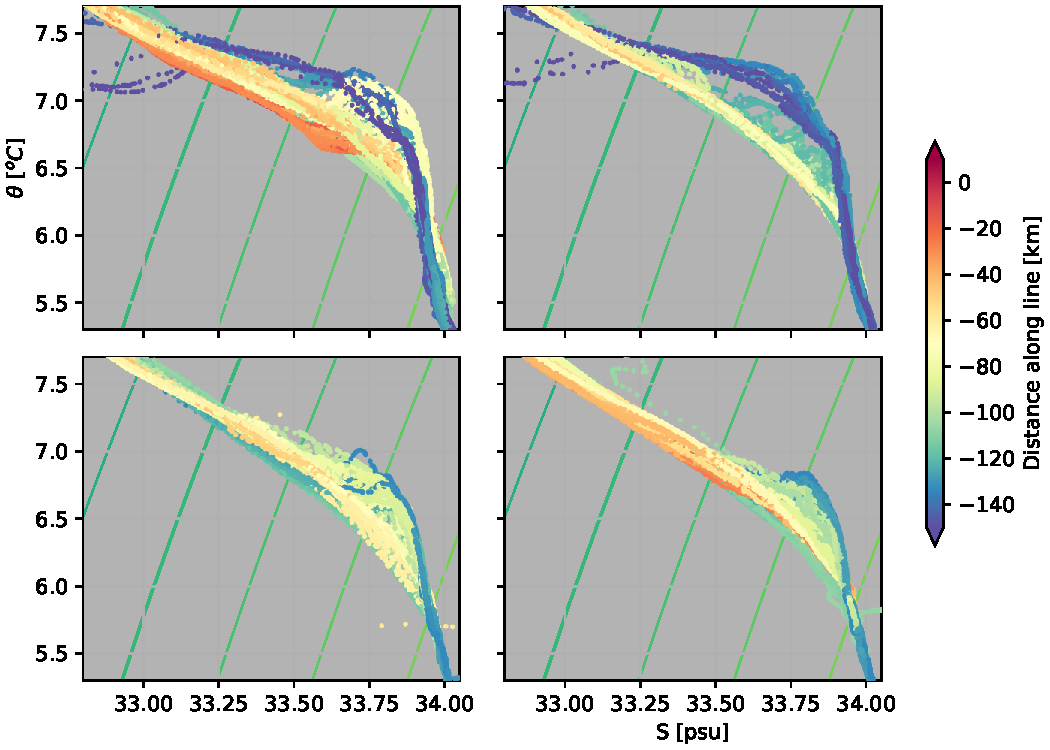
\includegraphics[width=\twowidth]{TSCanyon}
    \caption{
      \label{fig:TSCanyon} }
  \end{center}
\end{figure*}


\clearpage
\end{document}
